\documentclass[a4paper, 12pt]{article}
\usepackage[T2A]{fontenc}
\usepackage[utf8]{inputenc}
\usepackage[english,russian]{babel}
\usepackage{amsmath, amsfonts, amssymb, amsthm, mathtools, misccorr, indentfirst, multirow}
\usepackage{wrapfig}
\usepackage{graphicx}
\usepackage{subfig}
\usepackage{adjustbox}

\usepackage{geometry}
\geometry{top=20mm}
\geometry{bottom=20mm}
\geometry{left=20mm}
\geometry{right=20mm}

\title{Лабораторная работа 4.2.1\\Кольца Ньютона}
\author{Нехаев Александр\\654 группа}
\date{\today}

\begin{document}
	\maketitle
	\pagenumbering{gobble}
	\newpage
	\tableofcontents
	\pagenumbering{arabic}
	\newpage
	\section{Введение}
	\paragraph{Цель работы:} ознакомление с явлением интерференции в тонких пленках (полосы равной толщины) на примере колец Ньютона и с методикой интерференционных измерений кривизны стеклянной поверхности.
	\paragraph{В работе используются:} измерительный микроскоп с опак-иллюми-натором; плосковыпуклая линза; пластинка из черного стекла; ртутная лампа ПРК-4; щель; линзы; призма прямого зрения; объектная шкала.\par
	В нашей установке кольца Ньютона образуются при интерференции световых волн, отраженных от границ тонкой воздушной прослойки, заключенной между выпуклой поверхностью линзы и плоской стеклянной пластинкой (рис. \ref{calc_scheme}). Наблюдение ведется в отраженном свете.\par
	\begin{wrapfigure}{1}{5cm}
		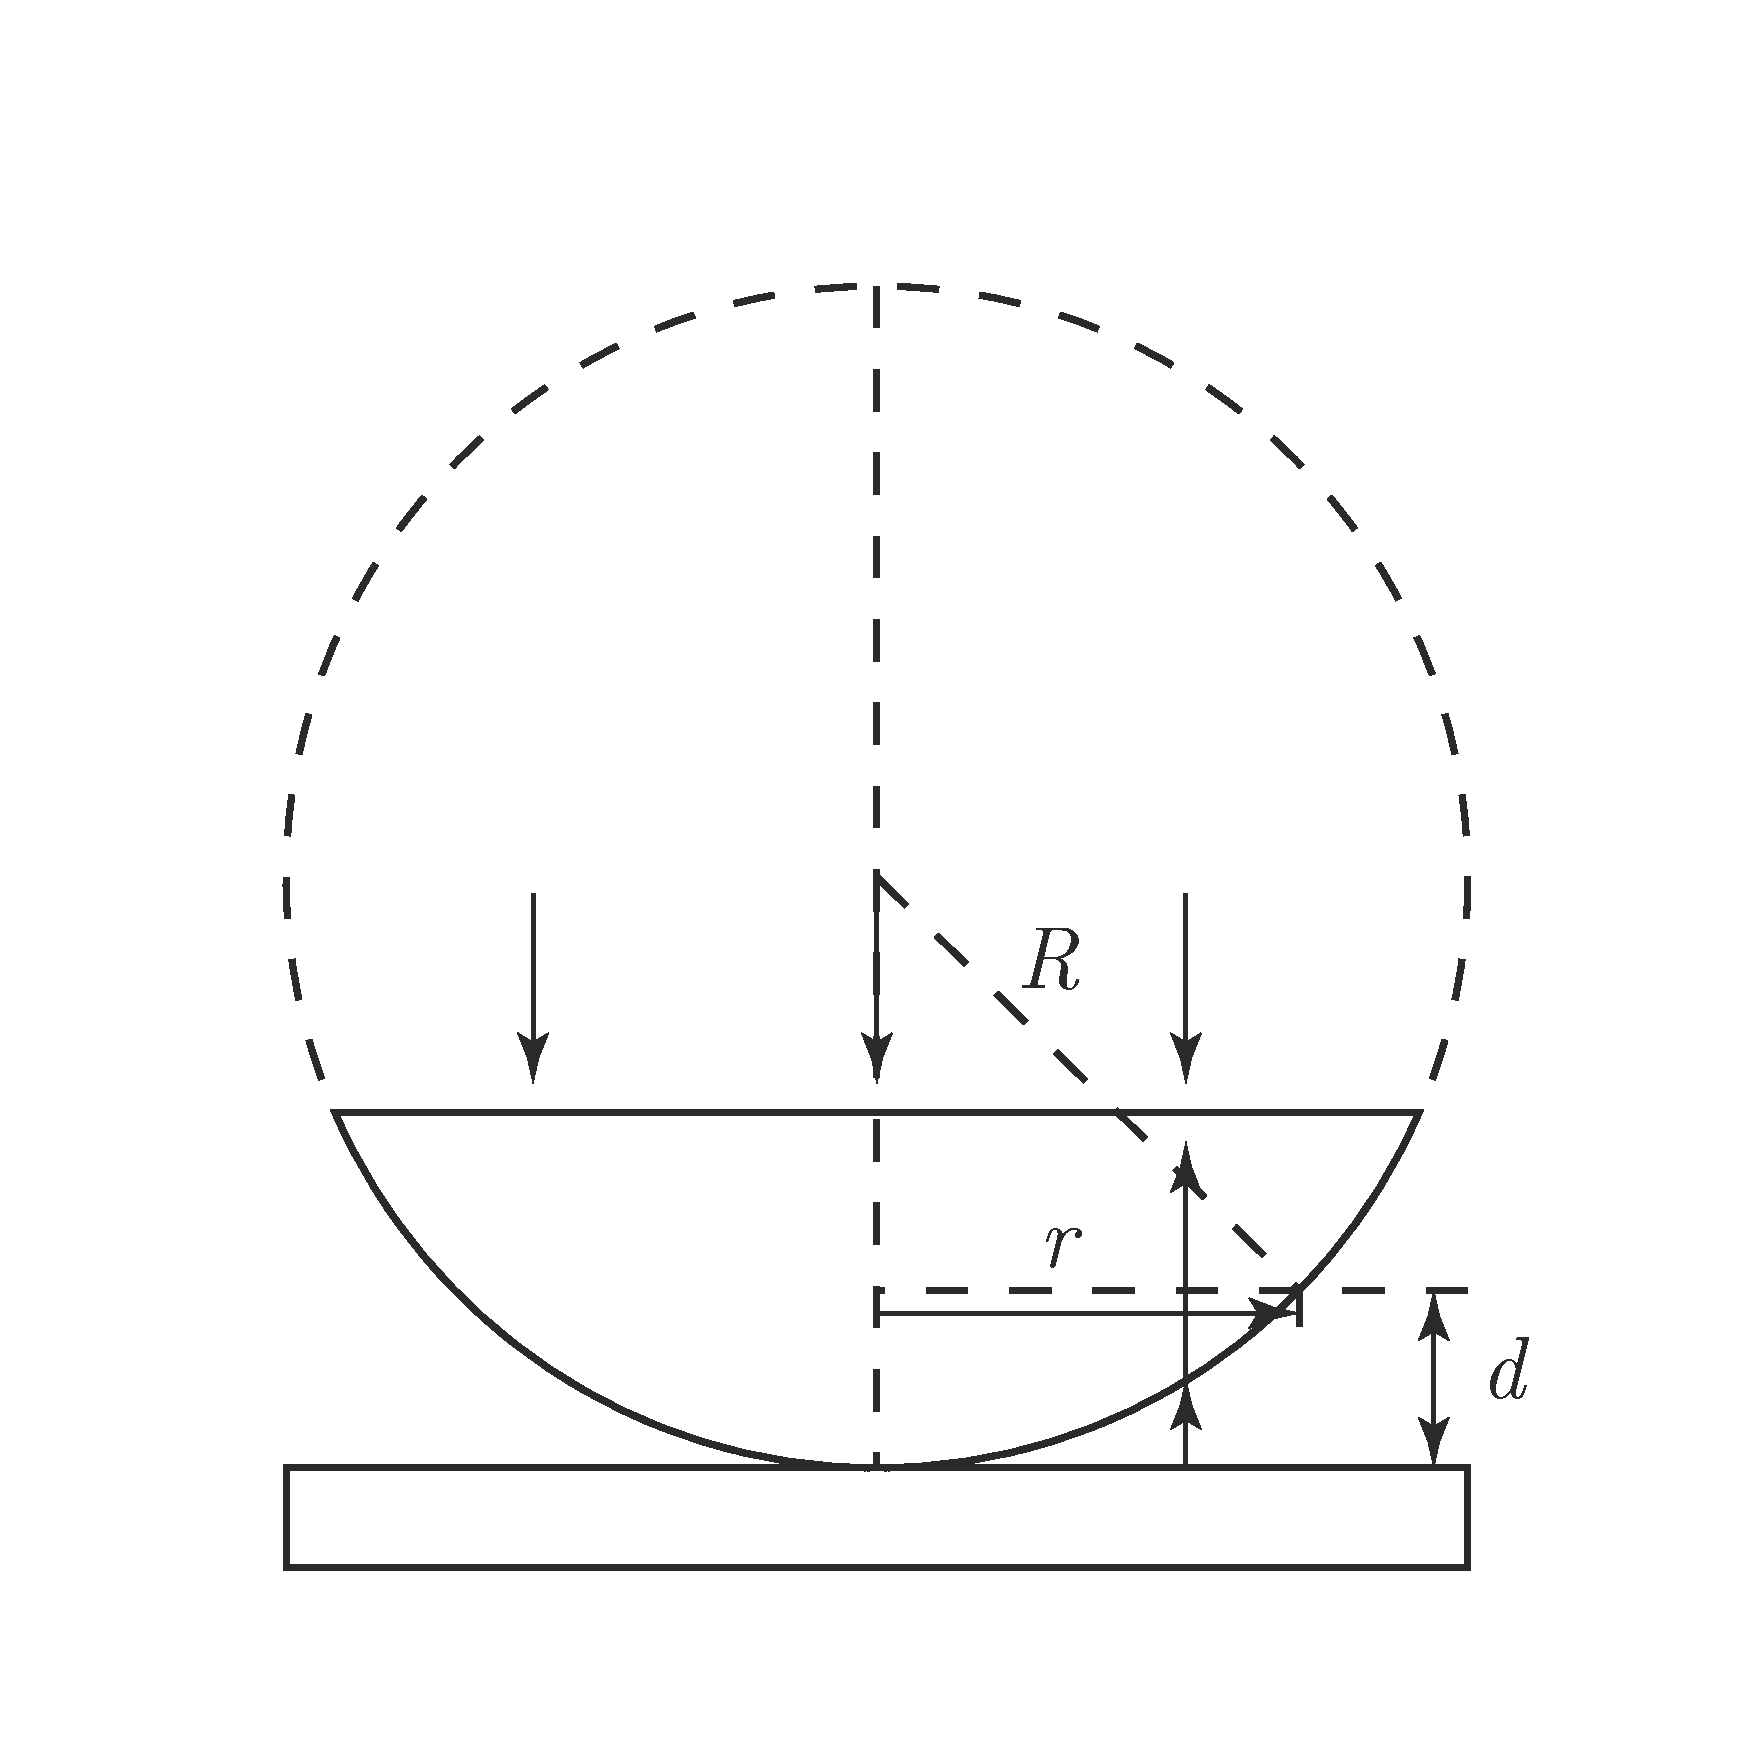
\includegraphics[scale=0.2]{Newton_Rings.pdf}
		\caption{К расчёту колец Ньютона}
		\label{calc_scheme}
	\end{wrapfigure}

	Рассчитаем размер колец Ньютона. Пусть сверху на линзу падает монохроматический параллельный пучок лучей. При вычислении разности хода можно пренебречь небольшими наклонами лучей, проходящих в тонком воздушном зазоре. Геометрическая разность хода между интерферирующими лучами равна, очевидно, $2d$, где $d$ — толщина воздушного зазора в данном месте.\par
	Выразим зависимость $d$ от расстояния $r$ до радиуса, проходящего через точку соприкосновения линзы и пластинки. Из рис. \ref{calc_scheme}. имеем
	\begin{equation*}
		r^2=R^2-\left(R-d\right)^2=2Rd-d^2,
	\end{equation*}
	где R — радиус кривизны выпуклой поверхности линзы. Принимая во внимание, что $2R\gg d$, получим
	\begin{equation}
		d=\frac{r^2}{2R}.
	\end{equation}
	\par
	При вычислении полной разности хода нужно учесть изменение фазы световой волны при отражении от границы стекло-воздух и воздух-стекло. Как известно, для светового (электрического) вектора отражение от оптически более плотной среды происходит с изменением фазы на $\pi$. Свет, отраженный от границы стекло—воздух, по сравнению со светом, отраженным от границы воздух—стекло, приобретает, таким образом, дополнительный фазовый сдвиг на $\pi$, что соответствует разности хода $\lambda/2$. Полная разность хода $\Delta$ равна
	\begin{equation}
		\Delta=2d+\frac{\lambda}{2}=\frac{r^2}{R}+\frac{\lambda}{2}.
		\label{way_delta_eq}
	\end{equation}
	Линии постоянной разности хода представляют собой концентрические кольца с центром в точке соприкосновения. При заданном значении длины волны $\lambda$ разность хода $\Delta$ определяется толщиной воздушного зазора; интерференционные полосы являются, таким образом, линиями равной толщины.\par
	Известно, что линии равной толщины для точечного источника света не имеют области локализации: их можно наблюдать в любом месте пространства, где пересекаются лучи, отражённые от двух поверхностей. Для протяжённого источника линии равной толщины локализованы на поверхности клина (в нашем случае на поверхности воздушной прослойки). Это означает, что при освещении системы не вполне параллельным пучком света (что практически всегда имеет место) интерференционные полосы оказываются наиболее четкими при фокусировке на верхнюю поверхность воздушного клина.\par
	Запишем условие минимума освещенности в интерференционной картине:
	\begin{equation}
		\Delta=\left(2m+1\right)\frac{\lambda}{2}, \quad m=0,1,2, ...
	\end{equation}
	Принимая во внимание (\ref{way_delta_eq}), получим для радиусов $r_m$ темных колец
	\begin{equation}
		r_m=\sqrt{mR\lambda}.
		\label{dark_ring_radius_eq}
	\end{equation}
	Аналогичным образом для радиусов $r_m'$ светлых колец найдем
	\begin{equation}
		r_m'=\sqrt{\left(2m-1\right)R\lambda/2}.
		\label{light_ring_radius_eq}
	\end{equation}
	\par
	Измеряя радиусы светлых или темных колец, с помощью (\ref{dark_ring_radius_eq}) и (\ref{light_ring_radius_eq}) можно определить $\lambda$, если известен радиус $R$ кривизны линзы, или, наоборот, по известному значению $\lambda$ найти $R$.
	\section{Экспериментальная установка}
	Опыт выполнятся с помощью измерительного микроскопа
\end{document}